\chapter{Methods}
This chapter contains a description of the methods used in describing the hardware on the FPGA side using \clash{} and VHDL. The description of the host-side (HPS) programming is included in appendix \ref{app:data_io}, as even though this part of the project is crucial for obtaining results, it is merely tangential to the project goals. 

\section{Overall structure}
In any reasonably complex project it pays off to keep a clear structure: it improves understandability and allows for easier debugging. For simple projects in \clash{}, the structure would be uniquely determined by the HDL generated by \clash{}, but this project also relies on other sources of HDL. Most noteworthy, the interface between the HPS and the FPGA; these signals are very specific to the type of the FPGA and the interconnects it has to the HPS. Luckily, the vendor (Altera) provides a way to generate HDL (the QSys system) in order to create a bridge from the host code running on the HPS to the programmable hardware, the FPGA. This process is described in appendix \ref{app:data_io_setup}. After configuring the bridge, VHDL can be generated and we are left with an instantiable VHDL component. However, even though \clash{} is capable of instantializing external IP components written in VHDL \cite{CLaSHBlogTut}, the most sensible way of implementing such a structure (due to the easy extensibility) is by writing a specific connecting component in VHDL, which can instantiate the \clash{}-generated VHDL. The only responsibility of the connecting component is to distribute and forward signals: it should not perform any computation. It would be a straightforward process of generating such a connecting component based on the signal names in the top-level entities of the components it instantiates, however, due to the fact that it does not change for different designs and it is not very large, the connecting component has been written by hand in VHDL. Figure \ref{f:large_structure} depicts an overview schematic of the complete system, including both the FPGA and HPS side.

\begin{figure}[h]
	\centering
	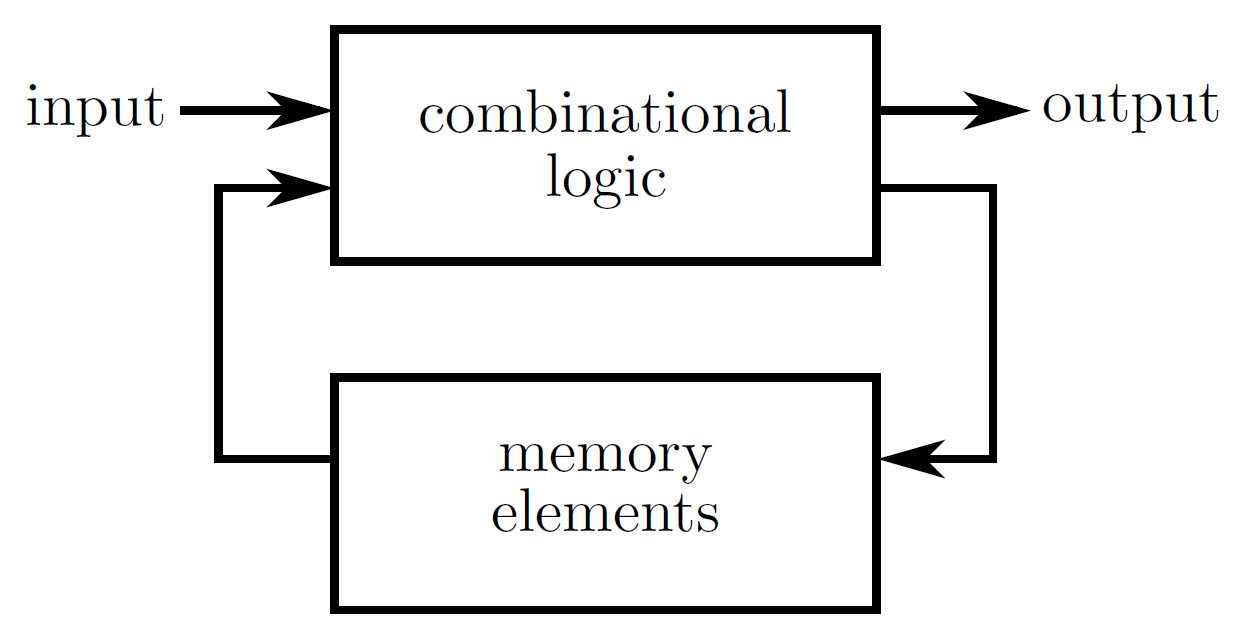
\includegraphics[width=\textwidth]{mealy_machine}
	\caption{TODO FIX ENTER GRAPHIC OF STRUCTURE WITH ILLUSTRATOR}
	\label{f:large_structure}
\end{figure}

\section{External types}
Usually, one of the first things to do when setting up a Haskell project is defining types, and using \clash{} forms no difference. It is especially useful to start by defining an input and an output signal. In a project with simple IO requirements the input and output signals would map straight to switches, keys and LEDs for testing purposes, but as the goal is to write data from the host system into the FPGA registers, the input and output signals will be a lot more complicated. The input and output signals from the \clash{}-generated VHDL top entity are shown in listing \ref{lst:clash_io_types}. The input consists of three separate channels: a bidirectional control channel, the actual input channel and some input needed for the output channel. It might appear strange that the output channel requires input, but this is necessary as the communications adhere to a strict master-slave pattern, in which the HPS is the master and the FPGA the slave. The HPS has to indicate whenever it wants to receive the FPGA output (by specifying an address (\code{out_address}) and setting the \code{out_read}-bit). As a consequence of the strict master-slave protocol, there are a lot less output signals than input signals: only the control and output channel can output data. Lastly, there are the keys, switches and LEDs as additional input and output signals. This concludes the type signatures of the input and output signals in \clash{}-Haskell. However, as the goal is to generate actual VHDL, \clash{} requires some additional information for the naming of the ports of the topEntity of the VHDL module. This is specified using the \code{topEntity}-annotation. In this case this annotation is not very interesting and it's merely a restatement of the input and output signal names, but when the \clash{}-generated VHDL should instantiate other VHDL-modules or use multiple clocks, the annotation can become more complex. It is shown in listing \ref{lst:clash_topentity}. 

\lstinputlisting[caption=Input and output signals for CλaSH, label=lst:clash_io_types, firstline=5,lastline=21]{../clash/SolverTypes.hs}
\lstinputlisting[caption=Signal names\, used in the CλaSH-generated topEntity VHDL module, label=lst:clash_topentity, firstline=8,lastline=29]{../clash/Solver.hs}

\section{Internal types}
So far the external types of the \clash{}-code have been covered, but the real work is done by the internal types: the types that keep track of the state of the system and allow it to do useful work. In order to allow for easy modifications to the types upon which the FPGA operates, they have been defined once and have been referenced everywhere else. This in combination with the property of the higher-order functions in \clash{} that they can operate on all vectors, regardless of length ensures that changing some internal types will not break the program.

\subsection{Internal number representation}
The solvers main data type is \code{type Data = SFixed 8 24}. The constructor \code{SFixed 8 24} stands for a signed fixed-point number, with 8 integer bits and 24 fractional bits. It uses the 2's complement signed number representation, meaning that an 8-bit integer part is capable of representing the integers in the range $[-128..127]$. The 24 fractional bits give this number representation a smallest representable unit of $2^{-24}$. This results in accuracy up to the 7th decimal place, which is similar to the IEEE 754 single precision floating point standard. The main reason for the use of fixed point integers is that \clash{} does not support floating point numbers yet, but additionally, fixed point representations are less demanding on FPGA area and result in a shorter critical path. Furthermore, the reason for choosing the total width of the number representation to be 32-bits is purely convenience: the input and output bridges are also 32 bits wide which allows you to send a single number per write or read. The \code{UInt} type acts as number representation in cases where only positive integer values are required, for instance in counters.

\subsection{SystemConstants and SystemState}
The \code{SystemConstants} keep track of the variables that do not change during the process of solving the ODE. It consists of a variety of constants that need values for the integration scheme (\code{maxtime}, \code{timestep} and \code{maxstep}). Furthermore, it may contain custom constants, which are passed to the equation to be approximated. This setup allows for (limited) changes to the equation by changing the constants at run-time without the time-consuming requirement of recompiling the entire FPGA side of the project.

Moving on to the data type which responsible for keeping track of the state of the system: the \code{SystemState}. This type has two fields: the \code{ODEState}, which is has the exact same function as the similarly named type in section \ref{s:numsolHaskell}: it keeps track of the values and the time in the numerical solver. It does this using a \code{valueVector} (of type \code{Vec 4 Data}) and a \code{time} variable (of type \code{Data}). The main difference between the type of the \code{ValueVector} in this implementation of \code{ODEState} and the one in section \ref{s:numsolHaskell} is that this one uses a vector instead of a list. In Haskell, lists can have any length (including infinite) whereas the \clash{}-vectors have a fixed length. This property is very important when generating VHDL, as all vector lengths have to be immutable and known at compile-time in order to compile the higher-order Haskell functions (eg. map) to VHDL and afterwards to hardware. 

The second field of the \code{SystemState} is a counter called \code{step}. Together with the \code{maxstep} field in \code{SystemConstants}, these govern the amount of output generated from the FPGA. A more elaborate explanation of the generation of output can be found in section \ref{s:compute}.

\lstinputlisting[caption=Internal state variables for CλaSH, label=lst:clash_internal_types, firstline=23,lastline=45]{../clash/SolverTypes.hs}

\section{Loading data into the FPGA}
\subsection{Constants}
\lstinputlisting[caption=Handling the input of the constants, label=lst:clash_constants, firstline=100,lastline=109]{../clash/Solver.hs}

The first step of getting the system to work is loading constants into the FPGA. These constants govern the time step, the maximum time for simulation, how much output to generate and it's possible to specify custom constants which can be used in the equations you are solving. In order to keep the system simple, these constants are sent over the control channel as the input channel is reserved for initial values. However, before covering the specifics of handling the constants, it is important to understand the behaviour of the signals originating from the bridge between the HPS and the FPGA first. Whenever the HPS program writes the 32-bits value $V$ to 8-bit address $A$, three things happen simultaneously, \code{control_writedata} takes on the value $V$, \code{control_address} gets set to address $A$ and \code{control_write} gets set to true. This set up means that it is possible to differentiate the target of the control input signal based on the value of the address. Only whenever \code{control_write} is true the control input value can be considered valid. Lastly, as Haskell is a strongly typed language, you cannot simply insert a \code{BitVector 32}, originating from \code{control_writedata} into a \code{Vec 4 (SFixed 8 24)}. You first have to cast or unpack the \code{BitVector 32} into a \code{SFixed 8 24}, which luckily does not pose any problems as they both consist of 32 bits.

The protocol for entering constants is depicted in table \ref{t:control_protocol}.

\begin{tabular}{l l l}
	\label{t:control_protocol}
	\textbf{Address} & \textbf{Function} &  \textbf{Specifics} \\
	0 	& Signaling flags 			& Writing 1 starts the computation \\
	& 				 				& Writing 2 performs a soft reset \\
	1 	& Maximal computation time 	& \\
	2 	& Time step 				& \\
	3 	& Step limit for blocking	& \\ 
	4+ 	& Custom constants 			& \\
\end{tabular}

\subsection{Initial values}
The initial values are loaded into the FPGA in the same way as the constants. The address designates the location at which the value should be stored. 
In order to understand how the data gets loaded into the FPGA registers it is important to  If this is the case, the \code{valueVector} of \code{ODEState} in the \code{SystemState} gets updated: the value at \code{in_address} gets replaced with \code{in_writedata}, which gets \code{unpack}'ed into the main data type used by the application. 

\lstinputlisting[caption=State machine responsible for controlling the solver, label=lst:clash_statemachine, firstline=77,lastline=98]{../clash/Solver.hs}



\section{Running computations and extracting data}
\label{s:compute}
The \code{step} of \code{SystemState} in listing \ref{lst:clash_internal_types} field takes a bit more explanation. Every time the integration scheme gets applied, the \code{step} variable gets incremented. At some point, the value of \code{step} becomes larger or equal than the \code{maxstep} field from the data type \code{SystemConstants}. Whenever this happens, the system blocks until you order it to start again by setting the value of \code{step} to 0. During the time that the system does not progress, you can read out the values of the system.




\subsection{Implementation of equations and integration schemes}

\subsection{Implementation of the equations}





